A rezolvens operátor definíciója
\begin{equation}
    \op{G}\left( E \right) = \left(E-\op{H}\right)^{-1} = \frac{1}{E-\op{H}}
\end{equation}
és ezen operátorhoz tartozó két változós függvény a Green-függény.
\begin{equation}
    G\left( x, y; E \right) = \Bra{x}\op{G}\left(E\right)\Ket{y}
\end{equation}
A Green-függvény név indokolt, és ennek a segítségével fogom meghatározni a Green-függvényeket konkrét esetben. A teljességi reláció beszúrásával látható, hogy a kvantummechanikai Green-függény megegyezik a differenciálegyenletek elméletéből ismert Green-függvénnyel.
\begin{equation}
    \left(E-\op{H}\right)\op{G}\left( E \right) = \op{I},
\end{equation}
azaz
\begin{equation}
    \int dx^\prime \Bra{x}\left(\op{H} - E\right) \Ket{x^\prime}\Bra{x^\prime} \op{G}\left( E \right)\Ket{y} = \Bra{x}\op{I}\Ket{y} = \delta \left(x - y\right).
\end{equation} 
A $\Bra{x}\left(\op{H} - E\right) \Ket{x^\prime}$ maggal vett konvolúció a $\op{H} - E$ operátor hatása, ezért
\begin{equation}
    \left(\op{H}_x - E\right) G\left(x, y; E\right) = \delta\left(x - y\right),
\end{equation}
amely a differenciálegyenletek elméletéből ismert Green-függvény definíciója. Ebben a konkrét esetben
\begin{equation}
    \left( -\frac{\hbar^2}{2m}\frac{\partial^2}{\partial x^2} + Fx - E \right) G\left(x, y; E\right) = \delta\left(x - y\right)
	\label{green:deltaeq}
\end{equation}
\subsubsection{Egzakt Green-függvény}
ami azt jelenti, hogy az $x < y$ tartományban
\begin{equation}
    G\left(x, y; E\right) = C_1 \Ai\left(\sqrt[3]{\frac{2mF}{\hbar^2}}x - \sqrt[3]{\frac{2m}{\hbar^2F^2}}E\right) + C_2 \Bi\left(\sqrt[3]{\frac{2mF}{\hbar^2}}x - \sqrt[3]{\frac{2m}{\hbar^2F^2}}E\right)
    \label{green:xy}
\end{equation}
illetve az $x > y$ tartományban
\begin{equation}
    G\left(x, y; E\right) = C_3 \Ai\left(\sqrt[3]{\frac{2mF}{\hbar^2}}x - \sqrt[3]{\frac{2m}{\hbar^2F^2}}E\right) + C_4 \Bi\left(\sqrt[3]{\frac{2mF}{\hbar^2}}x - \sqrt[3]{\frac{2m}{\hbar^2F^2}}E\right)
    \label{green:yx}
\end{equation}
, ahol a $C$ együtthatók függhetnek $y$ és $E$ értékétől. A $C$ együtthatók meghatározásához a doboz eredeti határfeltételeit $x = 0$ és $x = L$ pontban, valamint az $x = y$ pontban \aref{green:deltaeq}. egyenlet $y$ körüli integrálásából kapott feltételeket kell felhasználni. A doboz falára vonatkozó határfeltételek:
\begin{equation}
	\left. G\left(x,y;E\right)\right\rvert_{x = 0} = 0
\end{equation}
\begin{equation}
	\left. G\left(x,y;E\right)\right\rvert_{x = L} = 0
\end{equation}
\Aref{green:deltaeq}. egyenlet $\int_{y-\epsilon}^{y+\epsilon}\mathrm{d}x^\prime \int_{y}^{x^\prime} \mathrm{d}x$ szerinti integrálja az $\epsilon \to 0^+$ határesetben: 
\begin{equation}
	\lim_{\epsilon \to 0^+}\left.G\left(x,y;E \right)\right\rvert_{x = y - \epsilon}^{x = y + \epsilon} = 0
\end{equation}
A jobb oldal integrálja $\left. \left(x - y\right) \theta\left(x - y\right) \right\rvert_{x=y-\epsilon}^{x=y+\epsilon}$, ami a határesetben $0$. Az $\left(Fx - E\right)G\left(x,y;E\right)$ integrálja is $0$ a határesetben, mert az erdeti függvény is folytonos, így az integrálja is. \Aref{green:deltaeq}. egyenlet $x$ szerinti integrálja $y$ körüli $\epsilon$ sugarú környezetében az $\epsilon \to 0^+$ határesetben:
\begin{equation}
	\lim_{\epsilon \to 0^+}\left.\frac{\partial}{\partial x}G\left(x,y;E \right)\right\rvert_{x = y - \epsilon}^{x = y + \epsilon} = -\frac{2m}{\hbar^2}
\end{equation}
Itt a jobb oldal integrálja $\left. \theta\left(x - y\right) \right\rvert_{x = y - \epsilon}^{x = y + \epsilon} = 1$ a határesetben. A bal oldalon az előzőhöz hasonló módon csak a derivált integrálja marad meg. \Aref{green:xy}. és \aref{green:yx}. egyenlet behelyettesítése meghatározza a $C$ együtthatókra vonatkozó egyenleteket:
\begin{equation}
	\frac{C_2}{C_1} = -\Ti\left(-bE\right)
	\label{green:Cbegin}
\end{equation}
\begin{equation}
	\frac{C_4}{C_3} = -\Ti\left(aL - bE\right)
\end{equation}
\begin{equation}
	\frac{C_3}{C_1} = \frac{\Ti\left(ay - bE\right) - \Ti\left(-bE\right)}{\Ti\left(ay - bE\right) - \Ti\left(aL - bE\right)}
\end{equation}
TODO: $b$ lecserélése $bE$-re az előző részekben.
\begin{equation}
	C_1 = -\frac{2m}{a\hbar^2}\frac{1}{\left( \left(\frac{C_3}{C_1}-1\right)\Aip\left(ay - bE\right) + \left(\frac{C_4}{C_3}\frac{C_3}{C_1} - \frac{C_2}{C_1}\right) \Bip\left(ay - bE\right) \right)}
	\label{green:Cend}
\end{equation}
\begin{equation}
	C_1 = -\frac{a^2}{F}\frac{1}{\left( \left(\frac{C_3}{C_1}-1\right)\Aip\left(ay - bE\right) + \left(\frac{C_4}{C_3}\frac{C_3}{C_1} - \frac{C_2}{C_1}\right) \Bip\left(ay - bE\right) \right)}
\end{equation}
\Aref{green:Cbegin}-\ref{green:Cend}, \ref{green:xy}. és \aref{green:yx}. egyenletek explicit, analitikus módon előállítják a $G\left( x, y; E \right)$ Green-függvényt. Valós energiákra $G\left(x, y; E\right) = G\left(y, x; E\right)^*´$. Ebből következik, hogy a Green-függvény $x<y$ eset $y$ függése kiemelhető lesz, és megegyezik az $x>y$ eset $x$ függésével. Ezek szerint $\Ai\left(ay-bE\right)-\Ti\left(aL-bE\right)\Bi\left(ay-bE\right)$ kiemelhető a $C_1$ együtthatóból,
\begin{equation}
	C_1 = \frac{a^2}{F}\frac{\Ai\left(ay-bE\right)-\Ti\left(aL-bE\right)\Bi\left(ay-bE\right)}{\left(\Ti\left(-bE\right)-\Ti\left(aL-bE\right)\right)\left(\Bi\left(-bE\right)\Aip\left(-bE\right)-\Ai\left(-bE\right)\Bip\left(-bE\right)\right)}.
\end{equation}
Az algebrai átalakításokon túl fel kellett használni, hogy $\Ai\left(ay-bE\right)\Bip\left(ay-bE\right)-\Bi\left(y-bE\right)\Aip\left(ay-bE\right)$ $y$-tól független konstans tehát $y=0$ helyettesíthető bele. Ez onnan látható, hogy $y$ szerinti deriváltja $0$,
\begin{dmath}
	\left(\Ai\left(ay-bE\right)\Bip\left(ay-bE\right)-\Bi\left(ay-bE\right)\Aip\left(ay-bE\right)\right)^\prime = a\Ai^\prime\left(ay-bE\right)\Bi^\prime\left(ay-bE\right) + a\Ai\left(ay-bE\right)\Bi^{\prime\prime}\left(ay-bE\right) - a\Bi^\prime\left(ay-bE\right)\Ai^\prime\left(ay-bE\right) - a\Bi\left(ay-bE\right)\Ai^{\prime\prime}\left(ay-bE\right) = a\Ai\left(ay-bE\right)\left(ay-bE\right)\Bi\left(ay-bE\right) - a\Bi\left(ay-bE\right)\left(ay-bE\right)\Ai\left(ay-bE\right) = 0.
\end{dmath}
Ez után már az $x$-$y$ szimmetriája jól látható a Green-függvénynek.
\begin{equation}
	C_0 = \frac{a^2}{F}\frac{1}{\left(\Ti\left(-bE\right)-\Ti\left(aL-bE\right)\right)\left(\Bi\left(-bE\right)\Aip\left(-bE\right)-\Ai\left(-bE\right)\Bip\left(-bE\right)\right)}
\end{equation}
bevezetésével a Green függvény egyszerűbb alakra hozható,
\begin{equation}
	G\left(x,y;E\right) = C_0\times
	\begin{cases}
		\begin{split}
			\left(\Ai\left(ay-bE\right)-\Ti\left(aL-bE\right)\Bi\left(ay-bE\right)\right)\times\\
			\left(\Ai\left(ax-bE\right)-\Ti\left(-bE\right)\Bi\left(ax-bE\right)\right)
		\end{split} & x\leq y\\
		\begin{split}
			\left(\Ai\left(ay-bE\right)-\Ti\left(-bE\right)\Bi\left(ay-bE\right)\right)\times\;\;\;\;\;\;\;\;\\
			\left(\Ai\left(ax-bE\right)-\Ti\left(aL-bE\right)\Bi\left(ax-bE\right)\right)
		\end{split}& x>y\\
	\end{cases}
\end{equation} 

A rezolvens operátornak pólusai vannak a rendszer $E_k$ sajátenergiáinál:
\begin{equation}
	\op{G}\left(E\right) = \sum_n \frac{\Ket{n}\Bra{n}}{E_n - E}
	\label{green:greensum}
\end{equation}
Így ha $E$ kielégíti \aref{box_energiaszintek_egyenlet}. egyenletet, akkor a rezolvensnek és ezért a Green-függénynek is pólusa kell hogy legyen. Ezt a $C_1$ szingularitásán lehet a leg könnyebben belátni. Ha $C_1$ szinguláris, az összes többi $C$ együttható is, és így a Green-függvény is. \Aref{box_energiaszintek_egyenlet}. egyenlet szerint a $\frac{C_3}{C_1}$ számlálójának és nevezőének ,ásodik tagjai egyenlőek. Első tagjuk bármely $E$ esetén egyenlő, így  hányadosuk $1$, valamint \aref{box_energiaszintek_egyenlet}. egyenlet esetén $\frac{C_2}{C_1} = \frac{C_4}{C_3}$. Ezeknek a következtében mind $\frac{C_3}{C_1} - 1$, mind $\frac{C_4}{C_3}\frac{C_3}{C_1} - \frac{C_2}{C_1}$ $0$-val egyenlő, így a $C_1$-re vonatkozó kifejezés nevezője $0$. Ezek a $\frac{1}{E_n - E}$ típusú pólusok \aref{green:greensum}. egyenletből.

Egy érdekes matematikai eredmény, hogy a Green-függvényre vonatkozó differenciál egyenlet megoldásával elvégeztem \aref{green:greensum}. egyenlet összegzését. Ez az összeg az Airy függvények szorzatának összege lenne, osztva $E_k-E$-vel és a megfelelő normálási faktorral, ami Airy függvények szorzatának $0$ és $L$ közötti integrálj, valamint $E_k$-t \aref{box_energiaszintek_egyenlet}. transzcendens egyenlet határozza meg. A Green-függvényre vonatkozó differenciálegyenlet nélkül az összeg elvégzése reménytelennek látszana.

\begin{equation}
	\rho\left(E\right) = \frac{1}{\pi}\lim_{\epsilon \to 0^+} \mathrm{Im}\mathrm{Tr}\op{G}\left(E + i\epsilon\right)
	\label{green:densityeq}
\end{equation}
\begin{figure}[H]
	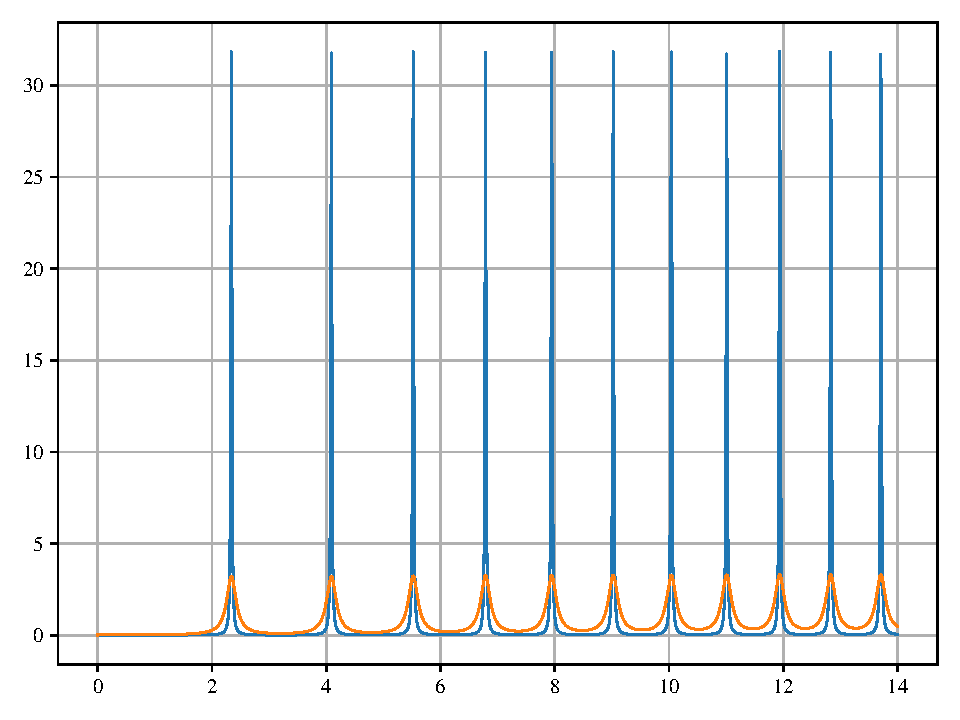
\includegraphics[scale=1]{./figs/dosfromgreen.pdf}
	\caption[Állapotsűrűség]{\Aref{green:densityeq}. képlet alapján számolt állapotsűrűség. A kék függvényt $\epsilon = 10^{-3}/b$, a narancssárga görbét pedig $\epsilon = 10^{-2}/b$ helyettesítéssel kaptuk. Látható, hogy $\epsilon$ csökkentésével a tüskék egyre keskenyebbek, és egyre magasabbak lesznek.}
	\label{green:állapotsűrség}
\end{figure}
\begin{figure}[H]
	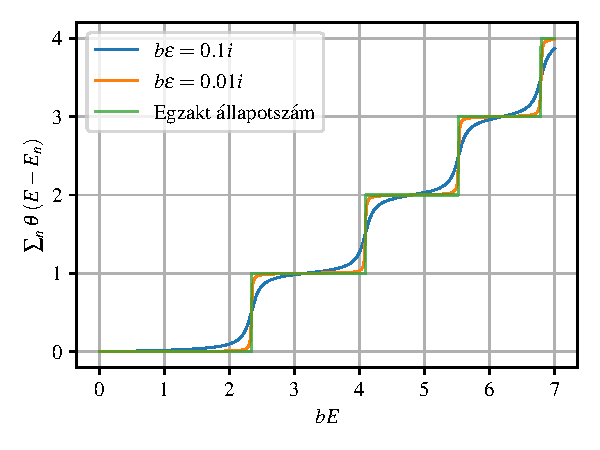
\includegraphics[scale=1]{./figs/numberofstatesfromgreen.pdf}
	\caption[Állapotok száma]{\Aref{green:állapotsűrség}. ábrán bemutatott függvények integrálja látható ezen az ábrán. Mind a két függvény ugrása közelítőleg $1$, ami at jelenti, hogy \aref{green:állapotsűrség}. ábrán látható tüskék alatti terület jó közelítéssel $1$. Az $\epsilon$ csökkentése a lépcsőfüggvényhez közelíti az integrált függvényt, ami egyezik az elvárásokkal.}
\end{figure}
\subsubsection{Green-függvény perturbáció számítással}
A perturbációszámításhoz a Hamilton operátort két részre bontom fel:
\begin{equation}
	\op{H} = \op{H}_0 + \op{V}
\end{equation}
A $\op{H}_0$ operátorhoz tartozó rezolvens $\op{G}_0\left(E\right)$. $\op{H}$ és $\op{H}_0$ kifejezhetőek a rezolvenseikkel. Ha a kifejezéseket behelyettesítjük a fenti egyenletbe, implicit egyenletet kapunk $op{G}\left(E\right)$-re nézve, melyet fel lehet használni perturbációszámításra. Az egyenletet balról $\op{G}_0^{-1}\left(E\right)$-vel, jobbról $\op{G}^{-1}\left(E\right)$-vel szorzunk.
\begin{equation}
	\op{G}^{-1}\left(E\right) + E = \op{G}_0^{-1}\left(E\right) + E + \op{V}
\end{equation}
\begin{equation}
	\op{G}\left(E\right) = \op{G}_0\left(E\right) - \op{G}_0\left(E\right)\op{V}\op{G}\left(E\right)
	\label{green:pertmaster}
\end{equation}
Az alábbi módon definiálva $\op{G}_n\left(E\right)$ operátort, \aref{green:pertmaster}. egyenlethez hasonló rekurziós összefüggés áll fent:
\begin{equation}
	\op{G}_n\left(E\right) = \op{G}_0\left(E\right)\sum_{k=0}^n\left(-\op{V}\op{G}_0\left(E\right)\right)^k
\end{equation}
\begin{equation}
	\op{G}_{n+1}\left(E\right) = \op{G}_0\left(E\right) - \op{G}_0\left(E\right)\op{V}\op{G}_n\left(E\right)
\end{equation}
Ha $\norm{\op{V}\op{G}_0\left(E\right)} < 1$ akkor a $\op{G}_n$ sorozat konvergál, és kielégíti \aref{green:pertmaster}. egyenletet. Ezért konvergencia esetén:
\begin{equation}
	\op{G}\left(E\right) = \op{G}_0\left(E\right)\sum_{n=0}^\infty\left(-\op{V}\op{G}_0\left(E\right)\right)^n
\end{equation}
A perturbbálatlan operátornak a lineáris potenciál nélküli dobozba zárt részecske Hamilton operátorát választom, $\op{H}_0=\frac{1}{2m}\op{p}^2$, így a lineáris potenciál marad a perturbáció $\op{V} = F\op{x}$. A perturbálatlan $\op{G}_0\left(E\right)$ Green-függvényt is \aref{green:Cbegin}-\ref{green:Cend}, \ref{green:xy}. és \aref{green:yx}. egyenletek alapján határozom meg.
\begin{equation}
	G_0\left(x,y;E\right) =
	\begin{cases}
		-\frac{2m}{k\hbar^2}\frac{1}{\sin\left(kL\right)} \sin\left(k\left(y-L\right)\right)\sin\left(kx\right) & x\leq y\\
		-\frac{2m}{k\hbar^2}\frac{1}{\sin\left(kL\right)} \sin\left(k\left(x-L\right)\right)\sin\left(ky\right) & x>y\\
	\end{cases}
\end{equation}
, ahol $k = \frac{\sqrt{2mE}}{\hbar}$.
\begin{figure}[H]
	\centering
	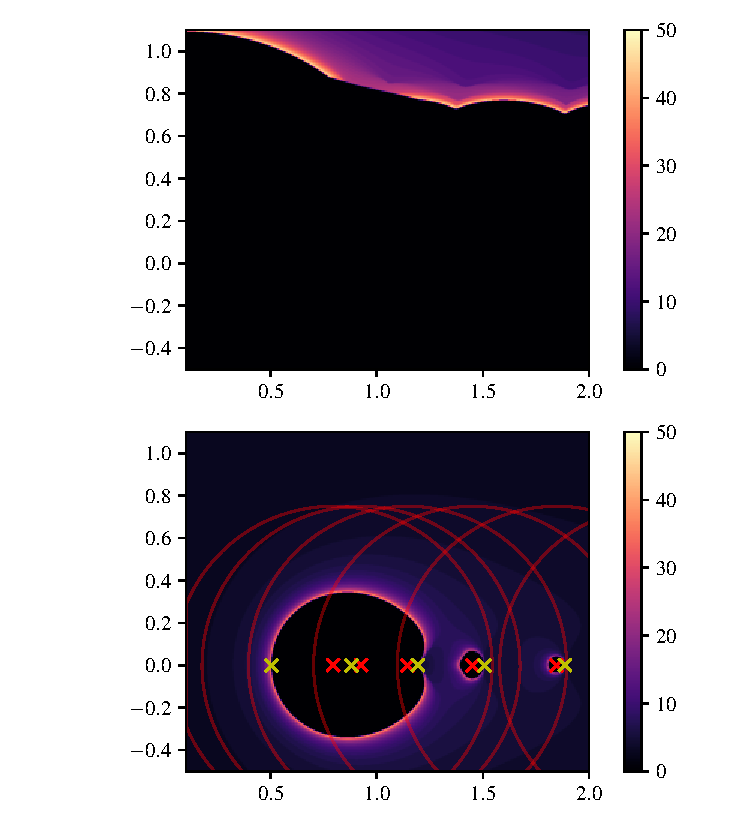
\includegraphics[scale=1]{./figs/convergence3.pdf}
	\caption[Green-függvény perturbációs sorának konvergenciája]{Ez az ábra a két perturbációs sor konvergenciáját hasonlítja össze a komplex energia síkon. A felső ábra a $V=Fx$ perturbáló potenciálnak, míg az alsó a $V = Fx-FL/2$ perturbáció szerinti sornak felel meg. A fekete tartományok divergenciát jelölnek, míg a többi szín a sorfejtés tagjainak csökkenési sebességét jellemzik, a norma harmadolásához szükséges lépések számát megadva. A piros körökön kívüli tartomány a ?? formula által garantált konvergencia tartományát jelöli. A piros x-ek a $\hat{G}_0$ pólusait, a sárga x-ek pedig az egzakt $\hat{G}$ operátor pólusait jelölik.}
\end{figure}






